% the following was taken from u-substitution

%\subsection*{Substitution and Inverse Trigonometric Functions}
%
%%In \autoref{sec:deriv_inverse_function} 
%When studying derivatives of inverse functions, we learned that $$\frac{d}{dx}\big(\tan^{-1}x\big) = \frac{1}{1+x^2}.$$ Applying the Chain Rule to this is not difficult; for instance, $$\frac{d}{dx}\big(\tan^{-1}5x\big) = \frac{5}{1+25x^2}.$$ We now explore how Substitution can be used to ``undo'' certain derivatives that are the result of the Chain Rule applied to Inverse Trigonometric functions. We begin with an example.\\
%
%\example{ex_subst14}{Integrating by substitution: inverse trigonometric functions}{
%Evaluate $\ds \int \frac{1}{25+x^2}\ dx$.}
%{The integrand looks similar to the derivative of the arctangent function. Note:
%\begin{align*}
%\frac{1}{25+x^2} &= \frac{1}{25(1+\frac{x^2}{25})}\\
%							&= \frac{1}{25(1+\left(\frac{x}{5}\right)^2)} \\
%							&= \frac{1}{25}\frac{1}{1+\left(\frac{x}{5}\right)^2}\ .
%\end{align*}
%Thus $$\int\frac{1}{25+x^2}\ dx = \frac{1}{25}\int \frac{1}{1+\left(\frac{x}{5}\right)^2}\ dx.$$ This can be integrated using Substitution. Set $u = x/5$, hence $du = dx/5$ or $dx=5du$. Thus
%\begin{align*}
%	\int\frac{1}{25+x^2}\ dx
%	&= \frac{1}{25}\int \frac{1}{1+\left(\frac{x}{5}\right)^2}\ dx \\
%	&= \frac15\int \frac{1}{1+u^2}\ du \\
%	&= \frac15\tan^{-1}u + C \\
%	&= \frac15\tan^{-1}\left(\frac x5\right)+C
%\end{align*}}
%
%\autoref{ex_subst14} demonstrates a general technique that can be applied to other integrands that result in inverse trigonometric functions. The results are summarized here.
%
%\theorem{thm:int_inverse_trig}{Integrals Involving Inverse Trigonomentric Functions}
%{Let $a>0$.
%\begin{enumerate}
%	\item	$\ds \int \frac{1}{a^2+x^2}\ dx = \frac1a\tan^{-1}\left(\frac{x}{a}\right) + C$
%	\item	$\ds \int \frac{1}{\sqrt{a^2-x^2}}\ dx = \sin^{-1}\left(\frac{x}{a}\right)+C$
%	\item	$\ds \int \frac{1}{x\sqrt{x^2-a^2}}\ dx = \frac1a\sec^{-1}\left(\frac{|x|}{a}\right)+C$
%\end{enumerate}}
%
%Let's practice using \autoref{thm:int_inverse_trig}.\bigskip
%
%\example{ex_subst15}{Integrating by substitution: inverse trigonometric functions}{Evaluate the given indefinite integrals.
%$$\int \frac{1}{9+x^2}\ dx,\quad \int \frac{1}{x\sqrt{x^2-\frac{1}{100}}}\ dx\quad \text{ and }\quad  \int \frac{1}{\sqrt{5-x^2}}\ dx.$$}
%{Each can be answered using a straightforward application of \autoref{thm:int_inverse_trig}.
%\begin{gather*}
%\int \frac{1}{9+x^2}\ dx = \frac13\tan^{-1} \frac x3 + C,\text{ as }a=3.
%\int\frac1{x\sqrt{x^2-\frac1{100}}}\ dx=10\sec^{-1}10x+C,\text{ as }a=\frac1{10}.
%\int \frac{1}{\sqrt{5-x^2}} = \sin^{-1}\frac{x}{\sqrt{5}}+C,\text{ as }a = \sqrt{5}.}
%
%Most applications of \autoref{thm:int_inverse_trig} are not as straightforward. The next examples show some common integrals that can still be approached with this theorem.\\
%
%\example{ex_subst16}{Integrating by substitution: completing the square}{Evaluate $\ds \int\frac{1}{x^2-4x+13}\ dx$.}
%{Initially, this integral seems to have nothing in common with the integrals in \autoref{thm:int_inverse_trig}. As it lacks a square root, it almost certainly is not related to arcsine or arcsecant. It is, however, related to the arctangent function.
%
%We see this by \textit{completing the square} in the denominator. We give a brief reminder of the process here. 
%
%Start with a quadratic with a leading coefficient of 1. It will have the form of $x^2 + bx + c$. Take 1/2 of $b$, square it, and add/subtract it back into the expression. I.e., 
%\begin{align*}
%	x^2+bx+ c
%	&= \underbrace{x^2 + bx + \frac{b^2}4}_{(x+b/2)^2} - \frac{b^2}4 + c\\
%	&= \left(x+\frac b2\right)^2 + c-\frac{b^2}4
%\end{align*}
%In our example, we take half of $-4$ and square it, getting $4$. We add/subtract it into the denominator as follows:
%
%\begin{align*}
%	\frac{1}{x^2-4x+13}
%	&= \frac{1}{\underbrace{x^2-4x+4}_{(x-2)^2}-4+13}\\
%	&=\frac{1}{(x-2)^2 + 9}
%\end{align*}
%We can now integrate this using the arctangent rule. Technically, we need to substitute first with $u=x-2$, but by now we can do this easily. Thus we have 
%\[
%\int \frac{1}{x^2-4x+13}\ dx
%= \int \frac{1}{(x-2)^2+9}\ dx
%= \frac13\tan^{-1}\frac{x-2}{3}+C.
%\]}
%
%\example{ex_subst17}{Integrals requiring multiple methods}{
%Evaluate $\ds \int \frac{4-x}{\sqrt{16-x^2}}\ dx$.}
%{This integral requires two different methods to evaluate it. We get to those methods by splitting up the integral: 
%\[
%\int \frac{4-x}{\sqrt{16-x^2}}\ dx
%= \int \frac{4}{\sqrt{16-x^2}}\ dx - \int \frac{x}{\sqrt{16-x^2}}\ dx.
%\]
%The first integral is handled using a straightforward application of \autoref{thm:int_inverse_trig}; the second integral is handled by substitution, with $u = 16-x^2$. We handle each separately.
%\[\int \frac{4}{\sqrt{16-x^2}}\ dx = 4\sin^{-1}\frac{x}{4} + C.\]
%For $\ds \int\frac{x}{\sqrt{16-x^2}}\ dx$, we set $u = 16-x^2$, so $du = -2xdx$ and $xdx = -du/2$. We have
%\begin{align*}
%	\int\frac{x}{\sqrt{16-x^2}}\ dx
%	&= \int\frac{-du/2}{\sqrt{u}}\\
%	&= -\frac12\int \frac{1}{\sqrt{u}}\ du \\
%	&= - \sqrt{u} + C\\
%	&= -\sqrt{16-x^2} + C.
%\end{align*}
%Combining these together, we have 
%\[\int \frac{4-x}{\sqrt{16-x^2}}\ dx = 4\sin^{-1}\frac x4 + \sqrt{16-x^2}+C.\]}


\section{Trigonometric Substitution}\label{sec:trig_sub}

In \autoref{sec:def_int} we defined the definite integral as the ``signed area under the curve.'' In that section we had not yet learned the Fundamental Theorem of Calculus, so we evaluated special definite integrals which described nice, geometric shapes. For instance, we were able to evaluate
\begin{equation}
\int_{-3}^3\sqrt{9-x^2}\ dx = \frac{9\pi}{2}\label{eq:trigsub1}
\end{equation}
 as we recognized that $f(x) = \sqrt{9-x^2}$ described the upper half of a circle with radius 3. 

We have since learned a number of integration techniques, including Substitution and Integration by Parts, yet we are still unable to evaluate the above integral without resorting to a geometric interpretation. This section introduces Trigonometric Substitution, a method of integration that fills this gap in our integration skill. This technique works on the same principle as Substitution as found in \autoref{sec:substitution}, though it can feel ``backward.'' In \autoref{sec:substitution}, we set $u=f(x)$, for some function $f$, and replaced $f(x)$ with $u$. In this section, we will set $x=f(\theta)$, where $f$ is a trigonometric function, then replace $x$ with $f(\theta)$. 

\youtubeVideo{yW6Odu0YHL0}{Trigonometric Substitution --- Example 3 / Part 1}

We start by demonstrating this method in evaluating the integral in \autoeqref{eq:trigsub1}. After the example, we will generalize the method and give more examples.

\example{ex_trigsub1}{Using Trigonometric Substitution}{Evaluate $\ds \int_{-3}^3\sqrt{9-x^2}\ dx$.}
{We begin by noting that $9\sin^2\theta + 9\cos^2\theta = 9$, and hence $9\cos^2\theta = 9-9\sin^2\theta$. If we let $x=3\sin\theta$, then $9-x^2 = 9-9\sin^2\theta = 9\cos^2\theta$. 

Setting $x=3\sin \theta$ gives  $dx = 3\cos\theta\ d\theta$. We are almost ready to substitute. We also change our bounds of integration. The bound $x=-3$ corresponds to $\theta = -\pi/2$ (for when $\theta = -\pi/2$, $x=3\sin \theta = -3$). Likewise, the bound of $x=3$ is replaced by the bound $\theta = \pi/2$. Thus
\begin{align*}
	\int_{-3}^3\sqrt{9-x^2}\ dx
	&= \int_{-\pi/2}^{\pi/2} \sqrt{9-9\sin^2\theta} (3\cos\theta)\ d\theta \\
	&= \int_{-\pi/2}^{\pi/2} 3\sqrt{9\cos^2\theta} \cos\theta\ d\theta \\
	&=\int_{-\pi/2}^{\pi/2} 3\abs{3\cos \theta} \cos\theta\ d\theta.
	\intertext{On $[-\pi/2,\pi/2]$, $\cos \theta$ is always positive, so we can drop the absolute value bars, then employ a half--angle formula:}
	&= \int_{-\pi/2}^{\pi/2} 9\cos^2 \theta\ d\theta\\
	&= \int_{-\pi/2}^{\pi/2} \frac{9}{2}\big(1+\cos(2\theta)\big)\ d\theta\\
	& = \frac92 \left.\left(\theta +\frac12\sin(2\theta)\right)\right|_{-\pi/2}^{\pi/2}= \frac92\pi.
\end{align*}
This matches our answer from before.}

We now describe in detail Trigonometric Substitution. This method excels when dealing with integrands that contain $\sqrt{a^2-x^2}$, $\sqrt{x^2-a^2}$ and $\sqrt{x^2+a^2}$. The following Key Idea outlines the procedure for each case, followed by more examples.
% Each right triangle acts as a reference to help us understand the relationships between $x$ and $\theta$.

\keyidea{idea:trigsub}{Trigonometric Substitution}
{\mbox{}\\[-2\baselineskip]\begin{enumerate}
	\item[(a)] \noindent%
		For integrands containing $\sqrt{a^2-x^2}$:\index{integration!trig. subst.}\smallskip\\
		Let $x=a\sin\theta$, \quad for $-\pi/2\leq \theta\leq \pi/2$. \smallskip\\
	On this interval, $\cos\theta\geq 0$, so	$\sqrt{a^2-x^2} = a\cos\theta$
		
	\item[(b)] \noindent
		For integrands containing $\sqrt{x^2+a^2}$:\smallskip\\
		Let $x=a\tan\theta$, \quad for $-\pi/2 < \theta < \pi/2$. \smallskip\\
	On this interval, $\sec\theta> 0$, so $\sqrt{x^2+a^2} = a\sec\theta$
		
	\item[(c)] \noindent
		For integrands containing $\sqrt{x^2-a^2}$:\smallskip\\
		Let $x=a\sec\theta$, \quad restricting our work to where $x\geq a$,\\
		so $x/a\geq 1$, and $0\leq\theta<\pi/2$. \smallskip\\
	On this interval, $\tan\theta\geq 0$, so	$\sqrt{x^2-a^2} = a\tan\theta$
\end{enumerate}}

\example{ex_trigsub3}{Using Trigonometric Substitution}{Evaluate $\ds \int \frac{1}{\sqrt{5+x^2}}\ dx.$}
{Using \autoref{idea:trigsub}(b), we recognize $a=\sqrt{5}$ and  set $x= \sqrt{5}\tan \theta$. This makes $dx = \sqrt{5}\sec^2\theta\ d\theta$. We will use the fact that $\sqrt{5+x^2} = \sqrt{5+5\tan^2\theta} = \sqrt{5\sec^2\theta} = \sqrt{5}\sec\theta.$ Substituting, we have:
\begin{align*}
\int \frac{1}{\sqrt{5+x^2}}\ dx &= \int \frac{1}{\sqrt{5+5\tan^2\theta}}\sqrt{5}\sec^2\theta\ d\theta \\
			&= \int \frac{\sqrt{5}\sec^2\theta}{\sqrt{5}\sec\theta} \ d\theta\\
			&= \int \sec\theta\ d\theta\\
			&= \ln\abs{\sec\theta+\tan\theta}+C.
\end{align*}
While the integration steps are over, we are not yet done. The original problem was stated in terms of $x$, whereas our answer is given in terms of $\theta$. We must convert back to $x$.

\mtable{A reference triangle for \autoref{ex_trigsub3}}{fig:tan_tri}{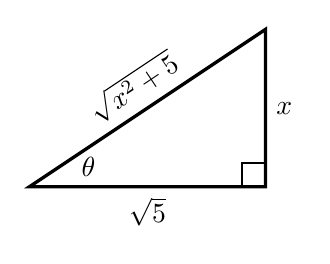
\begin{tikzpicture}
	\draw [very thick] (0,0) -- node[below,pos=.5] {$\sqrt5$} (3,0)
	 -- node [right,pos=.5] {$x$} (3,2)
	 -- node [pos=.5,above,sloped] {$\sqrt{x^2+5}$} cycle;
    \draw [thick] (2.7,0) -- (2.7,.3) -- (3,.3);
	\draw (.75,.25) node {$\theta$};
\end{tikzpicture}}
The reference triangle in \autoref{fig:tan_tri} will help. With $x=\sqrt{5}\tan\theta$, we have 
$$\tan \theta = \frac x{\sqrt{5}}\quad \text{and}\quad \sec\theta = \frac{\sqrt{x^2+5}}{\sqrt{5}}.$$
This gives
\begin{align*}
	\int\frac1{\sqrt{5+x^2}}\ dx
	&= \ln\abs{\sec\theta+\tan\theta}+C \\
	&= \ln\abs{\frac{\sqrt{x^2+5}}{\sqrt5}+ \frac x{\sqrt5}}+C.
\end{align*}
We can leave this answer as is, or we can use a logarithmic identity to simplify it. Note:
\begin{align*}
	\ln\abs{\frac{\sqrt{x^2+5}}{\sqrt5}+ \frac x{\sqrt5}}+C
	&= \ln\abs{\frac1{\sqrt5}\left(\sqrt{x^2+5}+ x\right)}+C \\
	&= \ln\abs{\frac1{\sqrt5}} + \ln\abs{\sqrt{x^2+5}+ x}+C\\
	&=	\ln\abs{\sqrt{x^2+5}+ x}+C,
\end{align*}
where the $\ln\big(1/\sqrt5\big)$ term is absorbed into the constant $C$. (In \autoref{sec:hyperbolic} we learned another way of approaching this problem.)}

\example{ex_trigsub2}{Using Trigonometric Substitution}{Evaluate $\ds \int \sqrt{4x^2-1}\ dx$.}
{We start by rewriting the integrand so that it looks like $\sqrt{x^2-a^2}$ for some value of $a$:
\begin{align*}
\sqrt{4x^2-1} &= \sqrt{4\left(x^2-\frac14\right)}\\
		&= 2\sqrt{x^2-\left(\frac12\right)^2}.
\end{align*}
So we have $a=1/2$, and following \autoref{idea:trigsub}(c), we set $x= \frac12\sec\theta$, and hence $dx = \frac12\sec\theta\tan\theta\ d\theta$. %The Key Idea also shows that $\sqrt{x^2-1/2^2} = \frac12\tan\theta$. 
We now rewrite the integral with these substitutions:
\begin{align*}
\int \sqrt{4x^2-1}\ dx &= \int 2\sqrt{x^2-\left(\frac12\right)^2}\ dx\\
			&= \int 2\sqrt{\frac14\sec^2\theta - \frac14}\left(\frac12\sec\theta\tan\theta\right)\ d\theta\\
			&=\int \sqrt{\frac14(\sec^2\theta-1)}\Big(\sec\theta\tan\theta\Big)\ d\theta\\
			&=\int\sqrt{\frac14\tan^2\theta}\Big(\sec\theta\tan\theta\Big)\ d\theta\\
			&=\int \frac12\tan^2\theta\sec\theta\ d\theta\\
			&=\frac12\int \Big(\sec^2\theta-1\Big)\sec\theta\ d\theta\\
			&=\frac12\int \big(\sec^3\theta - \sec\theta\big)\ d\theta.
\end{align*}
We integrated $\sec^3\theta$ in \autoref{ex_trigint6}, finding its antiderivatives to be
$$\int \sec^3\theta\ d\theta = \frac12\Big(\sec \theta\tan \theta + \ln|\sec \theta+\tan \theta|\Big)+C.$$
Thus
\flushinnerequ{%
\begin{align*}
\int \sqrt{4x^2-1}\ dx &=\frac12\int \big(\sec^3\theta - \sec\theta\big)\ d\theta\\
			&= \frac12\left(\frac12\Big(\sec \theta\tan \theta + \ln|\sec \theta+\tan \theta|\Big) -\ln|\sec \theta + \tan\theta|\right) + C\\
			%\end{align*}
			%\begin{align*}
			&= \frac14\left(\sec\theta\tan\theta -\ln|\sec\theta+\tan\theta|\right)+C.
\end{align*}}
We are not yet done. Our original integral is given in terms of $x$, whereas our final answer, as given, is in terms of $\theta$. We need to rewrite our answer in terms of $x$. With $a=1/2$, and $x=\frac12\sec\theta$, the reference triangle in \autoref{fig:sec_tri} shows that
\mtable{A reference triangle for \autoref{ex_trigsub2}}{fig:sec_tri}{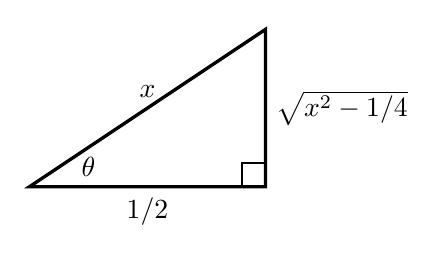
\begin{tikzpicture}
	\draw [very thick] (0,0) -- node[below,pos=.5] {$1/2$} (3,0)
	 -- node [right,pos=.5] {$\sqrt{x^2-1/4}$} (3,2)
	 -- node [pos=.5,above] {$x$} cycle;
    \draw [thick] (2.7,0) -- (2.7,.3) -- (3,.3);
	\draw (.75,.25) node {$\theta$};
\end{tikzpicture}}
$$\tan \theta = \frac{\sqrt{x^2-\frac14}}{\frac12} = 2\sqrt{x^2-\frac14}\qquad \text{and}\qquad\sec\theta = 2x.$$
Therefore,
\begin{align*}
	\int \sqrt{4x^2-1}\ dx
	& =\frac14\Big(\sec\theta\tan\theta -\ln\abs{\sec\theta+\tan\theta}\Big)+C \\
	&=\frac14\Big(2x\cdot 2\sqrt{x^2-\frac14} - \ln\abs{2x + 2\sqrt{x^2-\frac14}}\Big)+C\\
	&= \frac14\Big(4x\sqrt{x^2-\frac14}-\ln\abs{2x + 2\sqrt{x^2-\frac14}}\Big)+C \\
	& = \frac14\Big(2x\sqrt{4x^2-1} - \ln\abs{2x + \sqrt{4x^2-1}}\Big)+C.\eoehere
\end{align*}}

\example{ex_trigsub4}{Using Trigonometric Substitution}{Evaluate $\ds \int \frac{\sqrt{4-x^2}}{x^2}\ dx$.}
{We use \autoref{idea:trigsub}(a) with $a=2$, $x=2\sin \theta$, $dx = 2\cos \theta$ and hence $\sqrt{4-x^2} = 2\cos\theta$. This gives
\begin{align*}
\int \frac{\sqrt{4-x^2}}{x^2}\ dx &= \int \frac{2\cos\theta}{4\sin^2\theta}(2\cos\theta)\ d\theta\\
		&= \int \cot^2\theta\ d\theta\\
		&=	\int (\csc^2\theta -1)\ d\theta\\
		&= -\cot\theta -\theta + C.
\end{align*}
\mtable{A reference triangle for \autoref{ex_trigsub4}}{fig:sin_tri}{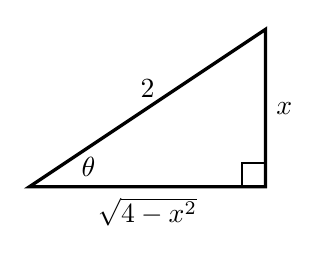
\begin{tikzpicture}
	\draw [very thick] (0,0) -- node[below,pos=.5] {$\sqrt{4-x^2}$} (3,0)
	 -- node [right,pos=.5] {$x$} (3,2) -- node [pos=.5,above] {$2$} cycle;
    \draw [thick] (2.7,0) -- (2.7,.3) -- (3,.3);
	\draw (.75,.25) node {$\theta$};
\end{tikzpicture}}
We need to rewrite our answer in terms of $x$. Using the reference triangle found in \autoref{fig:sin_tri}, we have $\cot\theta = \sqrt{4-x^2}/x$ and $\theta = \sin^{-1}(x/2)$. Thus
$$\int \frac{\sqrt{4-x^2}}{x^2}\ dx = -\frac{\sqrt{4-x^2}}x-\sin^{-1}\left(\frac x2\right) + C.\eoehere$$}

Trigonometric Substitution can be applied in many situations, even those not of the form $\sqrt{a^2-x^2}$, $\sqrt{x^2-a^2}$ or $\sqrt{x^2+a^2}$. In the following example, we apply it to an integral we already know how to handle.

\example{ex_trigsub5}{Using Trigonometric Substitution}{Evaluate $\ds \int\frac1{x^2+1}\ dx$.}
{We know the answer already as $\tan^{-1}x+C$. We apply Trig\-o\-no\-metric Substitution here to show that we get the same answer without inherently relying on knowledge of the derivative of the arctangent function.

Using \autoref{idea:trigsub}(b), let $x=\tan\theta$, $dx=\sec^2\theta\ d\theta$ and note that $x^2+1 = \tan^2\theta+1 = \sec^2\theta$. Thus
\begin{align*}
\int \frac1{x^2+1}\ dx &= \int \frac{1}{\sec^2\theta}\sec^2\theta\ d\theta \\
			&= \int 1\ d\theta\\
			&= \theta + C.
\end{align*}
Since $x=\tan \theta$, $\theta = \tan^{-1}x$, and we conclude that $\ds \int\frac1{x^2+1}\ dx = \tan^{-1}x+C.$}

The next example is similar to the previous one in that it does not involve a square--root. It shows how several techniques and identities can be combined to obtain a solution.

\example{ex_trigsub7}{Using Trigonometric Substitution}{Evaluate $\ds\int\frac1{(x^2+6x+10)^2}\ dx.$}
{We start by completing the square, then make the substitution $u=x+3$, followed by the trigonometric substitution of $u=\tan\theta$:
\begin{align}
\int \frac1{(x^2+6x+10)^2}\ dx =\int \frac1{\big((x+3)^2+1\big)^2}\ dx&= \int \frac1{(u^2+1)^2}\ du. \notag
\intertext{Now make the substitution $u=\tan\theta$, $du=\sec^2\theta\ d\theta$:}
   &=	\int \frac1{(\tan^2\theta+1)^2}\sec^2\theta\ d\theta\notag\\
	&= \int\frac 1{(\sec^2\theta)^2}\sec^2\theta\ d\theta\notag\\
	&= \int \cos^2\theta\ d\theta.\notag
	\intertext{Applying a half--angle formula, we have}
	&= \int \left(\frac12 +\frac12\cos(2\theta)\right)\ d\theta \notag\\
	&= \frac12\theta + \frac14\sin(2\theta) + C.\label{eq:extrigsub7}
\end{align}
\mnote{\textbf{Note:} Remember the sine and cosine double angle identities:
\begin{align*}
 \sin2\theta &= 2\sin\theta\cos\theta\\
 \cos2\theta &= \cos^2\theta-\sin^2\theta \\
 &= 2\cos^2\theta-1 \\
 &= 1-2\sin^2\theta
\end{align*}
They are often needed for writing your final answer in terms of $x$.}
We need to return to the variable $x$. As $u=\tan\theta$, $\theta = \tan^{-1}u$. Using the identity $\sin(2\theta) = 2\sin\theta\cos\theta$ and using the reference triangle found in \autoref{idea:trigsub}(b), we have 
$$\frac14\sin(2\theta) = \frac12\frac u{\sqrt{u^2+1}}\cdot\frac 1{\sqrt{u^2+1}} = \frac12\frac u{u^2+1}.$$
Finally, we return to $x$ with the substitution $u=x+3$. We start with the expression in \autoeqref{eq:extrigsub7}:
\begin{align*}
	\frac12\theta + \frac14\sin(2\theta) + C
	&= \frac12\tan^{-1}u + \frac12\frac{u}{u^2+1}+C\\
	&= \frac12\tan^{-1}(x+3) + \frac{x+3}{2(x^2+6x+10)}+C.
\end{align*}
Stating our final result in one line,
\[
\int\frac1{(x^2+6x+10)^2}\ dx=\frac12\tan^{-1}(x+3)+\frac{x+3}{2(x^2+6x+10)}+C.\eoehere
\]}

Our last example returns us to definite integrals, as seen in our first example. Given a definite integral that can be evaluated using Trigonometric Substitution, we could first evaluate the corresponding indefinite integral (by changing from an integral in terms of $x$ to one in terms of $\theta$, then converting back to $x$) and then evaluate using the original bounds. It is much more straightforward, though, to change the bounds as we substitute.

\example{ex_trigsub6}{Definite integration and Trigonometric Substitution}{Evaluate $\ds\int_0^5\frac{x^2}{\sqrt{x^2+25}}\ dx$.}
{Using \autoref{idea:trigsub}(b), we set $x=5\tan\theta$, $dx = 5\sec^2\theta\ d\theta$, and note that $\sqrt{x^2+25} = 5\sec\theta$. As we substitute, we change the bounds of integration.

The lower bound of the original integral is $x=0$. As $x=5\tan\theta$, we solve for $\theta$ and find $\theta = \tan^{-1}(x/5)$. Thus the new lower bound is $\theta = \tan^{-1}(0) = 0$. The original upper bound is $x=5$, thus the new upper bound is $\theta = \tan^{-1}(5/5) = \pi/4$. 

Thus we have 
\begin{align*}
\int_0^5\frac{x^2}{\sqrt{x^2+25}}\ dx &= \int_0^{\pi/4} \frac{25\tan^2\theta}{5\sec\theta}5\sec^2\theta\ d\theta\\
		&= 25\int_0^{\pi/4} \tan^2\theta\sec\theta\ d\theta.
\end{align*}
We encountered this indefinite integral in \autoref{ex_trigsub2} where we found 
$$\int \tan^2\theta\sec\theta \ d\theta = \frac12\big(\sec\theta\tan\theta-\ln|\sec\theta+\tan\theta|\big).$$
So
\begin{align*}
	25\int_0^{\pi/4} \tan^2\theta\sec\theta\ d\theta
	&= \left.\frac{25}2\left(\sec\theta\tan\theta-\ln\abs{\sec\theta+\tan\theta}\right)\right|_0^{\pi/4}\\
	&= \frac{25}2\big(\sqrt2-\ln(\sqrt2+1)\big)
%	\\
%	&\approx 6.661
	.\eoehere
\end{align*}}

%The following equalities are very useful when evaluating integrals using Trigonometric Substitution.
%
%\keyidea{idea:useful_trigsub}{Useful Equalities with Trigonometric Substitution}
%{\begin{enumerate}
%	\item	$\sin(2\theta) = 2\sin\theta\cos\theta$
%	\item	$\cos(2\theta) = \cos^2\theta - \sin^2\theta = 2\cos^2\theta-1 = 1-2\sin^2\theta$
%	\item $\ds \int \sec^3\theta\ d\theta = \frac12\Big(\sec \theta\tan \theta + \ln\big|\sec \theta+\tan \theta\big|\Big)+C$
%	\item	$\ds \int \cos^2\theta\ d\theta = \int \frac12\big(1+\cos(2\theta)\big)\ d\theta = \frac12\big(\theta+\sin\theta\cos\theta\big)+C.$
%\end{enumerate}}

The next section introduces Partial Fraction Decomposition, which is an algebraic technique that turns ``complicated'' fractions into sums of ``simpler'' fractions, making integration easier.

\printexercises{exercises/06_08_exercises}
